\documentclass[12pt]{article}
\usepackage{graphicx}
\usepackage{enumitem}
\usepackage{multicol}
\usepackage{mathtools}
\usepackage[margin=1in]{geometry}
\usepackage{amsmath,amsthm,amssymb}

 
\begin{document}
 
% --------------------------------------------------------------
%                         Start here
% --------------------------------------------------------------
 
\title{AST1430 Assignment 2}
\author{Jessica Campbell}
\date{February 20, 2018}
\maketitle

% --------------------------------------------------------------
%               1. LTE
% --------------------------------------------------------------

\section*{1. LTE}

This is preparation for Problem 2. An atom of two energy levels is immersed in a sea of electrons (of number density $n_e$ and kinetic temperature $T_K$), and bathed in a black-body background radiation (of radiation temperature $T_R$). This atom is excited both collisionally and radiatively. Define an excitation temperature ($T_s$, sometimes called the spin temperature when the transition concerns spin) by

\begin{align*}
\frac{n_2}{n_1} = \frac{g_2}{g_1}\exp\left(-\frac{\Delta E}{k_BT_s}\right)
\end{align*}

where $\Delta E = E_2 - E_1 > 0$ is the transition energy and $k_B$ the Stefan-Boltzman constant.

% --------------------------------------------------------------
%               Part 1)
% --------------------------------------------------------------

\subsection*{Part 1}

First write down the equation that describes the statistical equilibrium at which excitation and de-excitation of the upper level balances, and manipulate it to find

\begin{equation*}
\begin{split}
\exp\left(-\frac{\Delta E}{k_BT_s}\right) = \frac{\exp\left(-\frac{\Delta E}{k_BT_K}\right) + \frac{\xi}{\exp\left(\frac{\Delta E}{k_BT_R}\right)-1}} {1+\frac{\xi\exp\left(\frac{\Delta E}{k_BT_R}\right)}{\exp\left(\frac{\Delta E}{k_BT_R}\right)-1}}
\end{split}
\end{equation*}

where the dimensionless number $\xi = A_{21}/(n_eq_{21}) = A_{21}/(n_e\sigma_{21}v_e) = n_{crit}/n_e$. Here, $n_{crit}$ is the critical density for matter LTE.

% --------------------------------------------------------------
%               Solution
% --------------------------------------------------------------

\subsection*{Solution}

In statistical equilibrium, excitation balances de-excitation:

\begin{align*}
n_1n_eq_{12} + n_1\bar{J}B_{12} = n_2n_eq_{21} + n_2B_{21}\bar{J} + n_2A_{21}
\end{align*}

where $n_1$ and $n_2$ are the number densities of atoms in levels $1$ and $2$ respectively. In thermodynamic equilibrium, the ratio of these number densities follows the Boltzmann distribution:

\begin{align*}
\frac{n_2}{n_1} = \left(\frac{g_2}{g_1}\right)\exp\left(-\frac{\Delta E}{k_BT_S}\right).
\end{align*}

So, let's re-write the balance equation in a form that gives us $n_2/n_1$:

\begin{equation*}
\begin{split}
n_1n_eq_{12} + n_1\bar{J}B_{12} &= n_2n_eq_{21} + n_2B_{21}\bar{J} + n_2A_{21}\\
n_1( n_eq_{12} + \bar{J}B_{12} ) &= n_2( n_eq_{21} + B_{21}\bar{J} + A_{21} )\\
\frac{n_2}{n_1} &= \frac{ n_eq_{12} + \bar{J}B_{12}}{n_eq_{21} + B_{21}\bar{J} + A_{21}}
\end{split}
\end{equation*}

and now set this equal to the above Boltzmann equation:

\begin{align*}
\left(\frac{g_2}{g_1}\right)\exp\left(-\frac{\Delta E}{k_BT_S}\right) = \frac{ n_eq_{12} + \bar{J}B_{12}}{n_eq_{21} + B_{21}\bar{J} + A_{21}}.
\end{align*}

Dividing the top and bottom of the RHS by $(n_eq_{21})$, 

\begin{equation*}
\begin{split}
\left(\frac{g_2}{g_1}\right)\exp\left(-\frac{\Delta E}{k_BT_S}\right) &= \frac{ (n_eq_{12} + \bar{J}B_{12})/(n_eq_{21})}{(n_eq_{21} + B_{21}\bar{J} + A_{21})/(n_eq_{21})}\\
\left(\frac{g_2}{g_1}\right)\exp\left(-\frac{\Delta E}{k_BT_S}\right) &= \frac{ \frac{q_{12}}{q_{21}} + \frac{\bar{J}B_{12}}{n_eq_{21}} }{1 + \frac{B_{21}\bar{J}}{n_eq_{21}} + \frac{A_{21}}{n_eq_{21}}},
\end{split}
\end{equation*}

we can now use the fact that the ratio of collisional coefficients is given by:

\begin{align*}
\frac{q_{12}}{q_{21}} = \left(\frac{g_2}{g_1}\right)\exp\left(-\frac{\Delta E}{k_BT_K}\right).
\end{align*}

Substituting this for $q_{12}/q_{21}$ into our running balance equation:

\begin{equation*}
\begin{split}
\left(\frac{g_2}{g_1}\right)\exp\left(-\frac{\Delta E}{k_BT_S}\right) = \frac{ \left(\frac{g_2}{g_1}\right)\exp\left(-\frac{\Delta E}{k_BT_K}\right) + \frac{\bar{J}B_{12}}{n_eq_{21}} }{1 + \frac{B_{21}\bar{J}}{n_eq_{21}} + \frac{A_{21}}{n_eq_{21}}}.
\end{split}
\end{equation*}

In thermodynamic equilibrium, $\bar{J} \approx B_\nu(T)$ which can be written as:

\begin{align*}
\bar{J} = \frac{A_{21}/B_{21}}{\left(\frac{g_1B_{12}}{g_2B_{21}}\right)\exp\left(\frac{\Delta E}{k_BT_R}\right)-1}.
\end{align*}

Making this substitution for $\bar{J}$:

\begin{equation*}
\begin{split}
\left(\frac{g_2}{g_1}\right)\exp\left(-\frac{\Delta E}{k_BT_S}\right) &= \frac{ \left(\frac{g_2}{g_1}\right)\exp\left(-\frac{\Delta E}{k_BT_K}\right) + \left(\frac{A_{21}/B_{21}}{\left(\frac{g_1B_{12}}{g_2B_{21}}\right)\exp\left(\frac{\Delta E}{k_BT_R}\right)-1}\right) \frac{B_{12}}{n_eq_{21}} }{1 + \left(\frac{A_{21}/B_{21}}{\left(\frac{g_1B_{12}}{g_2B_{21}}\right)\exp\left(\frac{\Delta E}{k_BT_R}\right)-1}\right)\frac{B_{21}}{n_eq_{21}} + \frac{A_{21}}{n_eq_{21}}}\\
\left(\frac{g_2}{g_1}\right)\exp\left(-\frac{\Delta E}{k_BT_S}\right) &= \frac{ \left(\frac{g_2}{g_1}\right)\exp\left(-\frac{\Delta E}{k_BT_K}\right) + \left(\frac{B_{12}}{n_eq_{21}}\frac{A_{21}}{B_{21}}\frac{g_2B_{21}}{g_1B_{12}}\right)\left(\frac{1}{\exp\left(\frac{\Delta E}{k_BT_R}\right)-1}\right) }{1 + \left(\frac{B_{21}}{n_eq_{21}}\frac{A_{21}}{B_{21}}\frac{g_2B_{21}}{g_1B_{12}}\right)\left(\frac{1}{\exp\left(\frac{\Delta E}{k_BT_R}\right)-1}\right) + \frac{A_{21}}{n_eq_{21}}}\\
\left(\frac{g_2}{g_1}\right)\exp\left(-\frac{\Delta E}{k_BT_S}\right) &= \frac{ \left(\frac{g_2}{g_1}\right)\exp\left(-\frac{\Delta E}{k_BT_K}\right) + \left(\frac{A_{21}}{n_eq_{21}}\frac{g_2}{g_1}\right)\left(\frac{1}{\exp\left(\frac{\Delta E}{k_BT_R}\right)-1}\right) }{1 + \left(\frac{A_{21}}{n_eq_{21}}\frac{B_{21}g_2}{B_{12}g_1}\right)\left(\frac{1}{\exp\left(\frac{\Delta E}{k_BT_R}\right)-1}\right) + \frac{A_{21}}{n_eq_{21}}}.
\end{split}
\end{equation*}

From equations of detailed balance, we can use the fact that

\begin{align*}
\frac{B_{21}}{B_{12}} = \frac{g_1}{g_2}
\end{align*}

to substitute this for $(B_{21}/B_{12})$ into our equation:

\begin{equation*}
\begin{split}
\left(\frac{g_2}{g_1}\right)\exp\left(-\frac{\Delta E}{k_BT_S}\right) &= \frac{ \left(\frac{g_2}{g_1}\right)\exp\left(-\frac{\Delta E}{k_BT_K}\right) + \left(\frac{A_{21}}{n_eq_{21}}\frac{g_2}{g_1}\right)\left(\frac{1}{\exp\left(\frac{\Delta E}{k_BT_R}\right)-1}\right) }{1 + \left(\frac{A_{21}}{n_eq_{21}}\frac{g_1g_2}{g_2g_1}\right)\left(\frac{1}{\exp\left(\frac{\Delta E}{k_BT_R}\right)-1}\right) + \frac{A_{21}}{n_eq_{21}}}\\
\left(\frac{g_2}{g_1}\right)\exp\left(-\frac{\Delta E}{k_BT_S}\right) &= \frac{ \left(\frac{g_2}{g_1}\right)\exp\left(-\frac{\Delta E}{k_BT_K}\right) + \left(\frac{A_{21}}{n_eq_{21}}\frac{g_2}{g_1}\right)\left(\frac{1}{\exp\left(\frac{\Delta E}{k_BT_R}\right)-1}\right) }{1 + \left(\frac{A_{21}}{n_eq_{21}}\right)\left(\frac{1}{\exp\left(\frac{\Delta E}{k_BT_R}\right)-1}\right) + \frac{A_{21}}{n_eq_{21}}}\\
\left(\frac{g_2}{g_1}\right)\exp\left(-\frac{\Delta E}{k_BT_S}\right) &= \left(\frac{g_2}{g_1}\right) \frac{\exp\left(-\frac{\Delta E}{k_BT_K}\right) + \left(\frac{A_{21}}{n_eq_{21}}\right)\left(\frac{1}{\exp\left(\frac{\Delta E}{k_BT_R}\right)-1}\right) }{1 + \left(\frac{A_{21}}{n_eq_{21}}\right)\left(\frac{1}{\exp\left(\frac{\Delta E}{k_BT_R}\right)-1}\right) + \frac{A_{21}}{n_eq_{21}}}\\
\exp\left(-\frac{\Delta E}{k_BT_S}\right) &= \frac{\exp\left(-\frac{\Delta E}{k_BT_K}\right) + \left(\frac{A_{21}}{n_eq_{21}}\right)\left(\frac{1}{\exp\left(\frac{\Delta E}{k_BT_R}\right)-1}\right) }{1 + \left(\frac{A_{21}}{n_eq_{21}}\right)\left(\frac{1}{\exp\left(\frac{\Delta E}{k_BT_R}\right)-1}\right) + \frac{A_{21}}{n_eq_{21}}}.
\end{split}
\end{equation*}

Now, using the definition $\xi \equiv A_{21}/n_eq_{21}$ and rearranging terms:

\begin{equation*}
\begin{split}
\exp\left(-\frac{\Delta E}{k_BT_S}\right) &= \frac{\exp\left(-\frac{\Delta E}{k_BT_K}\right) + \xi\left(\frac{1}{\exp\left(\frac{\Delta E}{k_BT_R}\right)-1}\right) }{1 + \xi\left(\frac{1}{\exp\left(\frac{\Delta E}{k_BT_R}\right)-1}\right) + \xi}\\
\exp\left(-\frac{\Delta E}{k_BT_S}\right) &= \frac{\exp\left(-\frac{\Delta E}{k_BT_K}\right) + \left(\frac{\xi}{\exp\left(\frac{\Delta E}{k_BT_R}\right)-1}\right) }{1 + \xi\left(\frac{\exp\left(\frac{\Delta E}{k_BT_R}\right)-1+1}{\exp\left(\frac{\Delta E}{k_BT_R}\right)-1}\right)}\\
\exp\left(-\frac{\Delta E}{k_BT_S}\right) &= \frac{\exp\left(-\frac{\Delta E}{k_BT_K}\right) + \left(\frac{\xi}{\exp\left(\frac{\Delta E}{k_BT_R}\right)-1}\right) }{1 + \xi\left(\frac{\exp\left(\frac{\Delta E}{k_BT_R}\right)}{\exp\left(\frac{\Delta E}{k_BT_R}\right)-1}\right)}.
\end{split}
\end{equation*}

And now to take a moment to cry because I can't believe I typed that out.

% --------------------------------------------------------------
%               Part 2)
% --------------------------------------------------------------

\subsection*{Part 2}

Simplify the above expression to obtain that in the limits of $\xi \gg 1$, $T_s \approx T_R$; and when $\xi \ll 1$, $T_s \approx T_K$. Contemplate the meaning of these results.

% --------------------------------------------------------------
%               Solution
% --------------------------------------------------------------

\subsection*{Solution}

Starting with the equation we derived above:

\begin{equation*}
\begin{split}
\exp\left(-\frac{\Delta E}{k_BT_S}\right) &= \frac{\exp\left(-\frac{\Delta E}{k_BT_K}\right) + \left(\frac{\xi}{\exp\left(\frac{\Delta E}{k_BT_R}\right)-1}\right) }{1 + \xi\left(\frac{\exp\left(\frac{\Delta E}{k_BT_R}\right)}{\exp\left(\frac{\Delta E}{k_BT_R}\right)-1}\right)}\\
\exp\left(-\frac{\Delta E}{k_BT_S}\right) &= \frac{\exp\left(-\frac{\Delta E}{k_BT_K}\right) + \xi\left(\exp\left(\frac{\Delta E}{k_BT_R}\right)-1\right)^{-1} }{1 + \xi\exp\left(\frac{\Delta E}{k_BT_R}\right)\left(\exp\left(\frac{\Delta E}{k_BT_R}\right)-1\right)^{-1}}.
\end{split}
\end{equation*}

If $\xi\gg1$, the non-$\xi$ terms are negligible and can be ignored:

\begin{equation*}
\begin{split}
\exp\left(-\frac{\Delta E}{k_BT_S}\right) &\approx \frac{\xi\left(\exp\left(\frac{\Delta E}{k_BT_R}\right)-1\right)^{-1} }{\xi\exp\left(\frac{\Delta E}{k_BT_R}\right)\left(\exp\left(\frac{\Delta E}{k_BT_R}\right)-1\right)^{-1}}\\
\exp\left(-\frac{\Delta E}{k_BT_S}\right) &\approx \frac{1}{\exp\left(\frac{\Delta E}{k_BT_R}\right)}\\
\exp\left(-\frac{\Delta E}{k_BT_S}\right) &\approx \exp\left(-\frac{\Delta E}{k_BT_R}\right).
\end{split}
\end{equation*}

Therefore,

\begin{align*}
T_S \approx T_R.
\end{align*}

Now, if $\xi \ll 1$ the $\xi$ terms now become negligible:

\begin{equation*}
\begin{split}
\exp\left(-\frac{\Delta E}{k_BT_S}\right) \approx \frac{\exp\left(-\frac{\Delta E}{k_BT_K}\right)}{1}
\exp\left(-\frac{\Delta E}{k_BT_S}\right) \approx \exp\left(-\frac{\Delta E}{k_BT_K}\right).
\end{split}
\end{equation*}

Therefore,

\begin{align*}
T_S \approx T_K.
\end{align*}

% --------------------------------------------------------------
%               Part 3)
% --------------------------------------------------------------

\subsection*{Part 3}

Prove that if $T_K > T_R$, independent of the value of $\xi$, we have $T_s > T_R$. In other words, there cannot be absorption of the background radiation.

% --------------------------------------------------------------
%               Solution
% --------------------------------------------------------------

\subsection*{Solution}

I don't even know.

% --------------------------------------------------------------
%                    2. 21 cm Emission from the Early Universe
% --------------------------------------------------------------

\section*{2. 21 cm Emission From the Early Universe}

We apply results from the above problem to investigate the 21cm emission from the epoch of reionization (when all hydrogen in the intergalactic space is ionized by UV photons from, presumably, massive stars). The 21 cm transition is between two energy levels (one being the hydrogen ground state) split by the nucleus spin (so called hyper-fine transitions). $\Delta E$ when expressed in temperature equals 0.068 K. This is much smaller than $T_K$ or $T_R$. We ignore redshift effect in this problem.

% --------------------------------------------------------------
%               Part 1)
% --------------------------------------------------------------

\subsection*{Part 1}


For this transition, $A_{21} = 2.87 \times 10^{-15}$ s$^{-1}$, $g_2=3$ and $g_1=1$. Assume that $\sigma_{21}$ is of order (1 A)$^2$ and that $T_K=100$ K. What is your estimated value of $n_{crit}$? How does this compare with the mean baryon density of the universe $n_{baryon} \sim 10^{−6}(1+z)^3$ at re-ionization (currently thought to occur at $z \sim 10$)?

% --------------------------------------------------------------
%               Solution
% --------------------------------------------------------------

\subsection*{Solution}

The critical density can be found via:

\begin{align*}
n_{crit} \equiv \frac{A_{21}}{q_{21}} \equiv \frac{A_{21}}{\sigma_{21}v_e},
\end{align*}

so we just need to solve for $v_e$ by setting the kinetic energy equal to the thermal energy:

\begin{equation*}
\begin{split}
E_K &= E_{th}\\
\frac{1}{2}m_ev_e^2 &= \frac{3}{2}k_BT_K\\
v_e &= \sqrt{\frac{3k_BT_K}{m_e}}\\
v_e &= \sqrt{\frac{3(1.38\times10^{-23}\,\mathrm{J/K})(100\,\mathrm{K})}{9.11\times10^{-31}\,\mathrm{kg}}}\\
v_e &= 67430.70 \, \mathrm{m/s}.
\end{split}
\end{equation*}

We can now use this to calculate the critical density:

\begin{equation*}
\begin{split}
n_{crit} &\equiv \frac{A_{21}}{\sigma_{21}v_e}\\
n_{crit} &= \frac{2.87 \times 10^{-15}\,\mathrm{s}^{-1}}{(10^{-10}\,\mathrm{m})^2\,67430.70\,\mathrm{m/s}}\\
n_{crit} &= 4.26\times10^{-6}\,\mathrm{cm^{-3}}.
\end{split}
\end{equation*}

To compare it to the mean baryon density of the universe, let's first calculate $n_{baryon}$:

\begin{equation*}
\begin{split}
n_{baryon} &\sim 10^{-6}(1+z)^3\\
n_{baryon} &\sim 10^{-6}(11)^3\\
n_{baryon} &\sim 1.33\times10^{-3}\,\mathrm{cm^{-3}}.
\end{split}
\end{equation*}

The critical density of 21 cm emission is therefore much less than mean baryonic density of the universe, so it is in matter LTE.

% --------------------------------------------------------------
%               Part 2)
% --------------------------------------------------------------

\subsection*{Part 2}

Derive the following absorption coefficient for a clump of neutral hydrogen (number density $n_\mathrm{HI}$) in the 21 cm wavelength,

\begin{align*}
\alpha_\nu = \frac{3c^2A_{21}n_1}{8\pi\nu^2}\frac{0.068\,\mathrm{K}}{T_s}\phi(\nu) \approx \frac{3c^2A_{21}n_\mathrm{HI}}{32\pi\nu^2}\frac{0.068\,\mathrm{K}}{T_s}\phi(\nu),
\end{align*}

where $\phi(\nu)$ is the line profile function normalized as $\int_0^{\infty}\phi(\nu)d\nu=1$. The optical depth is the absorption coefficient integrated through the cloud, $\tau_\nu=\int\alpha_\nu ds$. Typically, $\tau_\nu\ll1$.


% --------------------------------------------------------------
%               Solution
% --------------------------------------------------------------

\subsection*{Solution}

Starting from the expression we derived for the absorption coefficient in the previous assignment:

\begin{equation*}
\begin{split}
\alpha_\nu &= \frac{c^2}{8\pi\nu^2}n_1A_{21}\left(\frac{g_2}{g_1}\right)\left(1-\exp\left(-\frac{\Delta E}{k_BT_s}\right)\right)\phi(\nu)\\
\alpha_\nu &= \frac{c^2}{8\pi\nu^2}n_1A_{21}\left(\frac{3}{1}\right)\left(1-\exp\left(-\frac{0.068\,\mathrm{K}}{T_s}\right)\right)\phi(\nu)\\
\alpha_\nu &= \frac{3c^2}{8\pi\nu^2}n_1A_{21}\left(1-\exp\left(-\frac{0.068\,\mathrm{K}}{T_s}\right)\right)\phi(\nu).
\end{split}
\end{equation*}

Assuming $0.068 \ll T_s$, we can do a Taylor expansion and disregard higher-order terms:

\begin{equation*}
\begin{split}
\alpha_\nu &= \frac{3c^2}{8\pi\nu^2}n_1A_{21}\left(1-\left(1-\frac{0.068\,\mathrm{K}}{T_s}\right)\right)\phi(\nu)\\
\alpha_\nu &= \frac{3c^2}{8\pi\nu^2}n_1A_{21}\left(\frac{0.068\,\mathrm{K}}{T_s}\right)\phi(\nu).
\end{split}
\end{equation*}

To convert $n_1$ into $n_\mathrm{HI}$, we can use the following as a substitution:

\begin{align*}
n_1 = \frac{n_\mathrm{HI}}{g_1+g_2} = \frac{n_\mathrm{HI}}{1+3} = \frac{n_\mathrm{HI}}{4}.
\end{align*}

Therefore,

\begin{equation*}
\begin{split}
\alpha_\nu &= \frac{3c^2}{8\pi\nu^2}\left(\frac{n_\mathrm{HI}}{4}\right)A_{21}\left(\frac{0.068\,\mathrm{K}}{T_s}\right)\phi(\nu)\\
\alpha_\nu &= \frac{3c^2}{32\pi\nu^2}n_\mathrm{HI}A_{21}\left(\frac{0.068\,\mathrm{K}}{T_s}\right)\phi(\nu).
\end{split}
\end{equation*}

% --------------------------------------------------------------
%               Part 3)
% --------------------------------------------------------------

\subsection*{Part 3}

Define a brightness temperature for the 21 cm emission, $T_b = T_b(\nu) = c^2/(2\nu^2k_B)\,I_\nu$. We are in the Rayleigh-Jeans limit ($h\nu = \Delta E k_BT$, where $T$ can be $T_s$, $T_b$, $T_R$ or $T_K$). Show that the source function $S_\nu \approx 2\nu^2/c^2k_BT_s$ and that this allows the equation of radiative transport to be simplified to the following form (eq. [1.61] in RL):

\begin{align*}
\frac{dT_b}{d\tau_\nu} = (T_s - T_b).
\end{align*}

Write down the solution for $T_b$ in terms of variables defined above. (\textit{Hint: the initial specific intensity originates from the radiation background.})

% --------------------------------------------------------------
%               Solution
% --------------------------------------------------------------

\subsection*{Solution}

Since the specific intensity originates from the radiation background, $S_\nu = B_\nu(T)$ so:

\begin{align*}
S_\nu = \frac{2h\nu^3}{c^2}\frac{1}{\exp\left(\frac{\Delta E}{k_BT_s}\right)-1}.
\end{align*}

Now, since we're in the Rayleigh-Jeans limit, $\Delta E \ll k_BT_s$ we can use a Taylor expansion to obtain the following simplification:

\begin{equation*}
\begin{split}
S_\nu &\approx \frac{2h\nu^3}{c^2}\frac{1}{\left(1+\frac{\Delta E}{k_BT_s}\right)-1}\\
S_\nu &\approx \frac{2h\nu^3}{c^2}\frac{1}{\left(\frac{\Delta E}{k_BT_s}\right)}\\
S_\nu &\approx \frac{2h\nu^3}{c^2}\left(\frac{k_BT_s}{\Delta E}\right).
\end{split}
\end{equation*}

Substituting $\Delta E=h\nu$ and simplifying for our final form:

\begin{equation*}
\begin{split}
S_\nu &\approx \frac{2h\nu^3}{c^2}\left(\frac{k_BT_s}{h\nu}\right)\\
S_\nu &\approx \frac{2\nu^2}{c^2}\left(\frac{k_BT_s}{1}\right)\\
S_\nu &\approx \left(\frac{2\nu^2k_B}{c^2}\right)T_s.
\end{split}
\end{equation*}

Turning to the canonical equation of radiative transfer,

\begin{align*}
\frac{dI_\nu}{d\tau} = S_\nu - I_\nu
\end{align*}

we just derived an expression for $S_\nu$ and we can use the definition of brightness temperature to obtain one for $I_\nu$:

\begin{equation*}
\begin{split}
T_b &\equiv T_b(\nu) = \frac{c^2}{2\nu^2k_B}I_\nu\\
I_\nu &= \left(\frac{2\nu^2k_B}{c^2}\right)T_b.
\end{split}
\end{equation*}

Substituting these into the equation of radiative transfer we obtain the following simplification:

\begin{equation*}
\begin{split}
\frac{d}{d\tau}\left(\frac{2\nu^2k_B}{c^2}T_b\right) &= \left(\frac{2\nu^2k_B}{c^2}\right)T_s - \left(\frac{2\nu^2k_B}{c^2}\right)T_b\\
\left(\frac{2\nu^2k_B}{c^2}\right) \frac{d}{d\tau}\left(T_b\right) &= \left(\frac{2\nu^2k_B}{c^2}\right)T_s - \left(\frac{2\nu^2k_B}{c^2}\right)T_b\\
\frac{dT_b}{d\tau} &= T_s - T_b.
\end{split}
\end{equation*}

To find the solution of $T_b$, we simply need to solve the differential equation:

\begin{equation*}
\begin{split}
\frac{dT_b}{d\tau} &= T_s - T_b\\
\frac{dT_b}{T_s - T_b} &= d\tau\\
\int_{T_{b_0}}^{T_b}\frac{dT_b}{T_s - T_b} &= \int_0^{\tau} d\tau.
\end{split}
\end{equation*}

Introducing a change of variables where $x \equiv T_s - T_b$ such that $dx=-dT_b$ and solving for $T_b$:

\begin{equation*}
\begin{split}
\int_{T_s-T_{b_0}}^{T_s-T_b}-\frac{dx}{x} &= \int_0^{\tau} d\tau\\
\int_{T_s-T_{b_0}}^{T_s-T_b}\frac{dx}{x} &= -\int_0^{\tau} d\tau\\
\ln(x)\rvert_{T_s-T_{b_0}}^{T_s-T_b} &= -\tau\rvert_0^{\tau}\\
\ln(T_s-T_{b_0}) - \ln(T_s-T_b) &= -\tau\\
\ln\left(\frac{T_s-T_b}{T_s-T_{b_0}}\right) &= -\tau\\
\exp\left[\ln\left(\frac{T_s-T_b}{T_s-T_{b_0}}\right)\right] &= \exp(-\tau)\\
\left(\frac{T_s-T_b}{T_s-T_{b_0}}\right) &= \exp(-\tau)\\
T_s-T_b &= (T_s-T_{b_0})\exp(-\tau)\\
T_b &= (T_{b_0}-T_s)\exp(-\tau) + T_s\\
T_b &= T_s(1-\exp(-\tau)) + T_{b_0}\exp(-\tau).
\end{split}
\end{equation*}

% --------------------------------------------------------------
%               Part 4)
% --------------------------------------------------------------

\subsection*{Part 4}

Radio telescopes will be able to measure 21cm emission from the early universe by detecting excess temperature over the CMB,

\begin{align*}
\delta T_b = T_b - T_R.
\end{align*}

Show that this excess is independent of the actual spin temperature as long as it lies sufficiently far above $T_R$ (currently at 2.7 K). This measurement allows one to obtain a good estimate of the $\mathrm{HI}$ column density as a function of redshift, thereby probing the processes occurring during reionization.

References for Problems 1 & 2:
Field, 1958, Proc. IRE, 46, 240 (original, no electronic version available)
Field, 1959, ApJ, 129,525 (visionary work)
Zaldarriaga et al 2004, ApJ, 608, 622 (recent analytical development)

% --------------------------------------------------------------
%               Solution
% --------------------------------------------------------------

\subsection*{Solution}

Starting with the solution that we just found for $T_b$:

\begin{align*}
T_b = T_s(1-\exp(-\tau)) + T_{b_0}\exp(-\tau),
\end{align*}

we can calculate $\delta T_b$ as follows:

\begin{equation*}
\begin{split}
\delta T_b = T_b - T_R
\delta T_b = T_s(1-\exp(-\tau)) + T_{b_0}\exp(-\tau) - T_R.
\end{split}
\end{equation*}

Since we know that $\tau \equiv \int\alpha_\nu ds$, this implies that $\tau_\nu \propto \alpha_\nu \propto 1/T_s$, so:

\begin{align*}
\delta T_b \sim T_s\left(1-\exp\left(-\frac{1}{T_s}\right)\right) + T_{b_0}\exp\left(-\frac{1}{T_s}\right) - T_R.
\end{align*}

If the spin temperature lies sufficiently far above the background radiation temperature, $T_s \gg T_R$, then $1/T_s \ll 1$ so we can perform a Taylor expansion:

\begin{equation*}
\begin{split}
\delta T_b &\approx T_s\left(1-\left[1-\frac{1}{T_s}\right]\right) + T_{b_0}\left[1-\frac{1}{T_s}\right] - T_R\\
\delta T_b &\approx T_s\left(\frac{1}{T_s}\right) + T_{b_0}\left[1-\frac{1}{T_s}\right] - T_R\\
\delta T_b &\approx 1 + T_{b_0}\left[1-\frac{1}{T_s}\right] - T_R\\
\delta T_b &\approx 1 + T_{b_0}(1) - T_R\\
\delta T_b &\approx 1 + T_{b_0} - T_R.
\end{split}
\end{equation*}

Therefore, $\delta T_b$ is independent of the spin temperature $T_s$.

% --------------------------------------------------------------
%                    4. Emission Line Fluxes
% --------------------------------------------------------------

\section*{4. Emission Line Fluxes}

Atomic and molecular infrared transitions are important for cooling the interstellar gas. One example for this is the cooling of metallic gas in the debris disk around
stars like $\beta$ Pictoris and others. The gas is largely ionized (except for $\mathrm{OI}$ which has a first ionization potential 16 eV) and is hydrogen-depleted. The gas is mostly composed of oxygen and carbon and has a mean ion/electron density of $\sim$ 10 cm$^{-3}$. Ignore carbon here.

% --------------------------------------------------------------
%               Part 1)
% --------------------------------------------------------------

\subsection*{Part 1}

The ground-state of $\mathrm{OI}$ (which has a configuration of $2s^22p^4$) is split by spin-orbit coupling to three. Transitions between these produce the $\mathrm{OI}$ 44 $\mu$m, 63.2 $\mu$m and 145.6 $\mu$m lines. Assuming LTE, which transition is most important for cooling the gas when gas temperature $T \sim$ 300 K? What about when $T \sim$ 50 K? For an $\mathrm{OI}$ number density of 1 cm$^{-3}$ and LTE, a gas temperature of 300 K, calculate the cooling luminosity from individual lines radiated by a cubic centimeter of material.

% --------------------------------------------------------------
%               Solution
% --------------------------------------------------------------

\subsection*{Solution}

Figure \ref{fig:table1} summarizes the three $\mathrm{OI}$ transitions: Earth, atmosphere and space:

\begin{figure}[h] \label{fig:table1}
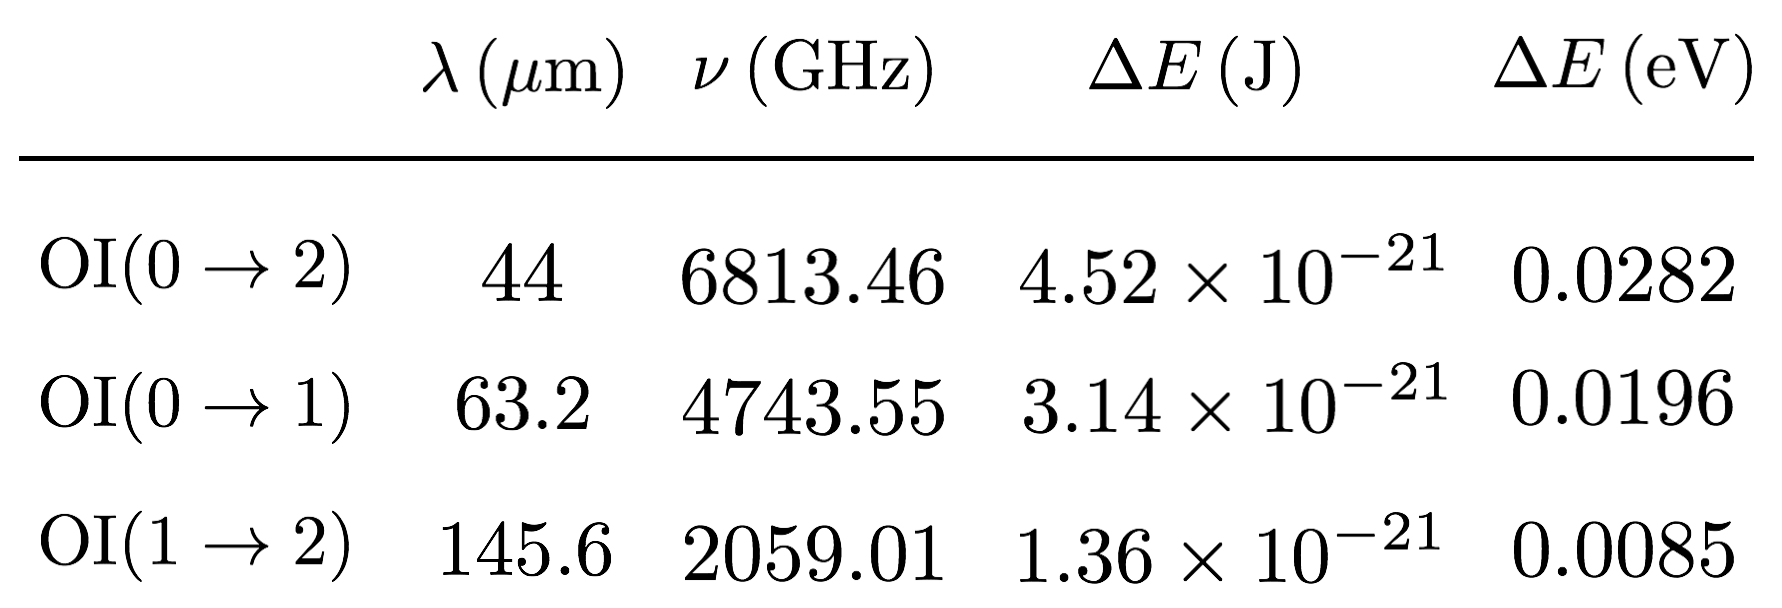
\includegraphics[width=8cm]{table1.png}
\centering
\caption{Summary of transitions.}
\end{figure}

{\noindent}\textbf{Gas Cooling}

To determine which transition dominates gas cooling, we must simply find the transitional energy that is closest to the value of $k_BT$ for the gas. For a gas temperature of $T\sim300\,\mathrm{K}$, $(k_BT)=4.14\times10^{-21}\,\mathrm{J} = 0.0259\,\mathrm{eV}$ so $\mathrm{OI(0\rightarrow1)}$ dominates the gas cooling. Similarly, for a gas temperature of $T\sim50\,\mathrm{K}$, $(k_BT)=6.903\times10^{-22}\,\mathrm{J} = 0.0043\,\mathrm{eV}$ so $\mathrm{OI(1\rightarrow2)}$ dominates the gas cooling.

{\noindent}\textbf{Cooling Luminosity}

For radiative cooling via emission lines such as the three $\mathrm{OI}$ transitions, atoms occupy two different energy levels $i$ and $j$ separated by an energy of $\Delta E_{ji}$. The Einstein coefficient $A_{ji}$ characterizes the rate of spontaneous emission from state $j\rightarrow i$ which have respective number densities of $n_j$ and $n_i$.

\begin{figure}[h] \label{fig:ji}
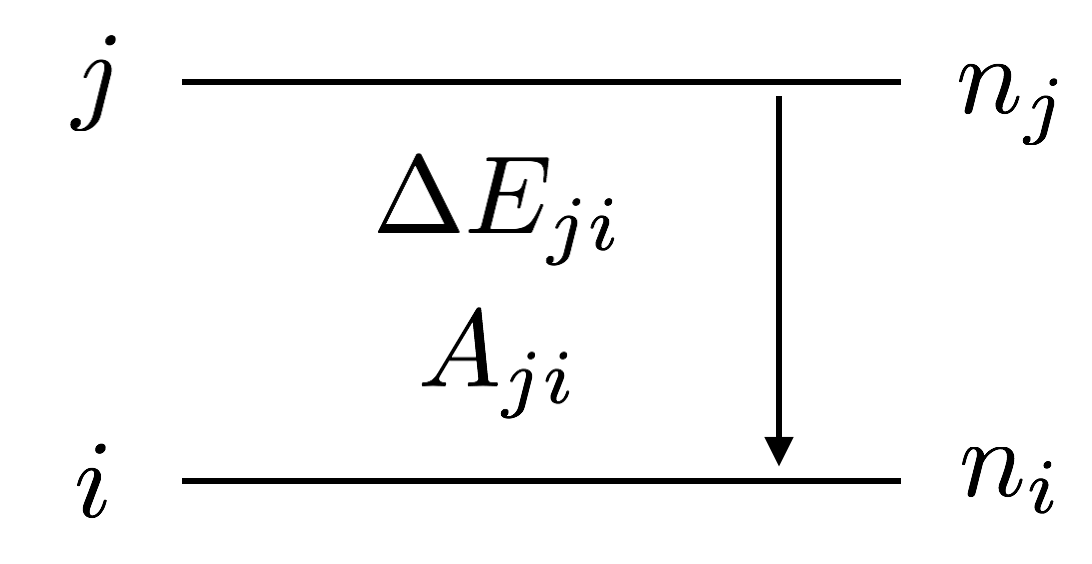
\includegraphics[width=8cm]{ji.png}
\centering
\caption{Schematic of energy transitions.}
\end{figure}

The cooling luminosity of a transition from state $j \rightarrow i$ in a volume $V$ is given by:

\begin{align*}
L_{ji} = n_j A_{ji}\Delta E_{ji}V.
\end{align*}

We're given that the total $\mathrm{OI}$ number density is $1\,\mathrm{cm^{-3}}$, but in order to determine a cooling luminosity for each of the transitions independently, we must solve for the independent number densities of the three states. Here, we can use the Boltzmann equation which relates two states $i$ and $j$:

\begin{align*}
\frac{n_j}{n_i} = \left(\frac{g_j}{g_i}\right)\exp\left(\frac{\Delta E_{ji}}{k_BT}\right).
\end{align*}

This allows us to relate the two number densities $n_1$ and $n_2$ to $n_0$ as such:

\begin{equation*}
\begin{split}
n_1 &= n_0\left(\frac{g_1}{g_0}\right)\exp\left(\frac{\Delta E_{10}}{k_BT}\right)\\
n_2 &= n_0\left(\frac{g_2}{g_0}\right)\exp\left(\frac{\Delta E_{20}}{k_BT}\right)
\end{split}
\end{equation*}

which allows to solve for $n_0$:

\begin{align*}
n_0 + n_1 + n_2 = 1 \, \mathrm{cm^{-3}}\\
n_0 + n_0\left(\frac{g_1}{g_0}\right)\exp\left(\frac{\Delta E_{10}}{k_BT}\right) + n_0\left(\frac{g_2}{g_0}\right)\exp\left(\frac{\Delta E_{20}}{k_BT}\right) = 1 \, \mathrm{cm^{-3}}\\
n_0 \left[1 + \left(\frac{g_1}{g_0}\right)\exp\left(\frac{\Delta E_{10}}{k_BT}\right) + \left(\frac{g_2}{g_0}\right)\exp\left(\frac{\Delta E_{20}}{k_BT}\right)\right] = 1 \, \mathrm{cm^{-3}}\\
n_0 = \frac{1\,\mathrm{cm^{-3}}}{1 + \left(\frac{g_1}{g_0}\right)\exp\left(\frac{\Delta E_{10}}{k_BT}\right) + \left(\frac{g_2}{g_0}\right)\exp\left(\frac{\Delta E_{20}}{k_BT}\right)}.
\end{align*}

To compute $n_0$, we must first obtain the transitional information from NIST.

\newpage

The following table summarizes the transitional information from NIST:

\begin{figure}[h] \label{fig:table2}
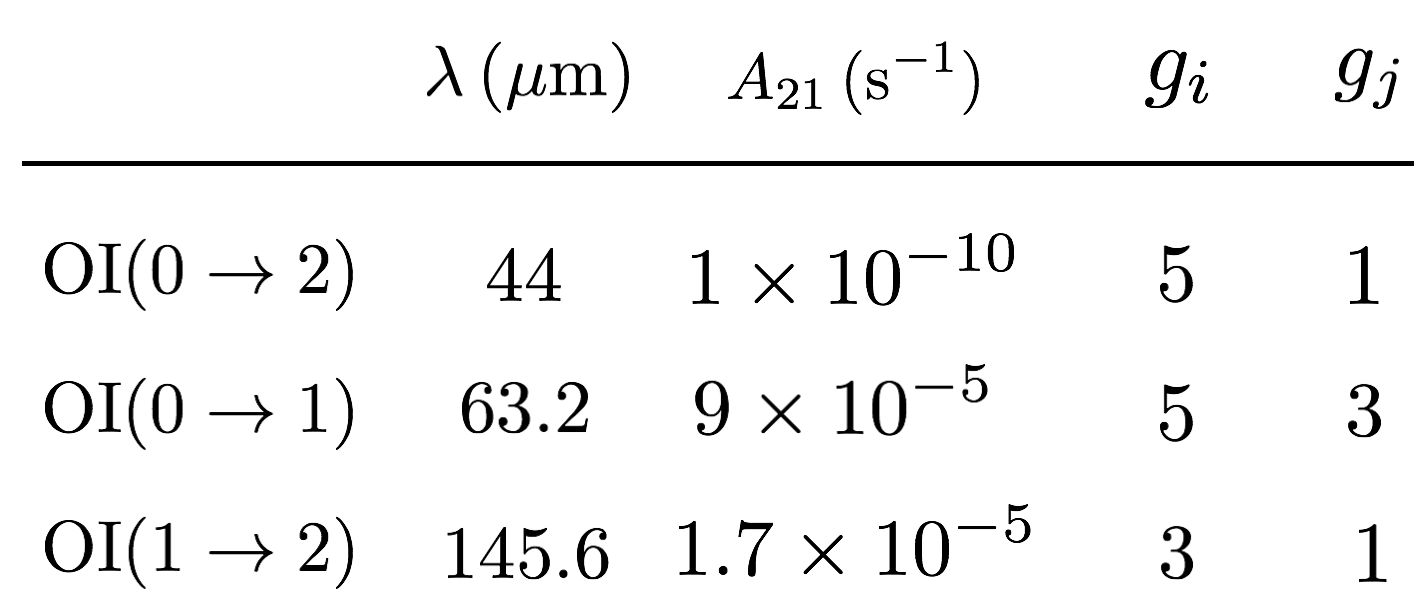
\includegraphics[width=8cm]{table2.png}
\centering
\caption{NIST results.}
\end{figure}

Using this transitional information along with $T=300\,\mathrm{K}$, we can now solve for $n_0$:

\begin{equation*}
\begin{split}
n_0 &= \frac{1\,\mathrm{cm^{-3}}}{1 + \left(\frac{g_1}{g_0}\right)\exp\left(\frac{\Delta E_{10}}{k_BT}\right) + \left(\frac{g_2}{g_0}\right)\exp\left(\frac{\Delta E_{20}}{k_BT}\right)}\\
n_0 &= \frac{1\,\mathrm{cm^{-3}}}{1 + \left(\frac{3}{5}\right)\exp\left(\frac{0.0196\,\mathrm{eV}}{k_B(300\,\mathrm{K})}\right) + \left(\frac{1}{5}\right)\exp\left(\frac{0.0282\,\mathrm{eV}}{k_B(300\,\mathrm{K})}\right)}\\
n_0 &= 0.35\,\mathrm{cm^{-3}}.
\end{split}
\end{equation*}

We can now return to the Boltzmann equations to determine the remaining number densities:

\begin{equation*}
\begin{split}
n_1 &= n_0\left(\frac{g_1}{g_0}\right)\exp\left(\frac{\Delta E_{10}}{k_BT}\right) = 0.35\,\mathrm{cm^{-3}}\left(\frac{3}{5}\right)\exp\left(\frac{0.019\,\mathrm{eV}}{k_B(300\,\mathrm{K})}\right) = 0.45\,\mathrm{cm^{-3}}\\
n_2 &= n_0\left(\frac{g_2}{g_0}\right)\exp\left(\frac{\Delta E_{20}}{k_BT}\right) = 0.35\,\mathrm{cm^{-3}}\left(\frac{1}{5}\right)\exp\left(\frac{0.0282\,\mathrm{eV}}{k_B(300\,\mathrm{K})}\right) = 0.21\,\mathrm{cm^{-3}}
\end{split}
\end{equation*}

We can now use these densities to calculate the cooling luminosity of each transition:

\begin{equation*}
\begin{split}
L_{20} &= n_2A_{20}\Delta E_{20}V = (0.21\,\mathrm{cm^{-3}})(1\times10^{-10}\,\mathrm{s^{-1}})(0.0282\,\mathrm{eV})(1\,\mathrm{cm^3}) = 5.84\times10^{-13} \,\mathrm{eV/s}\\
L_{10} &= n_1A_{10}\Delta E_{10}V = (0.45\,\mathrm{cm^{-3}})(9\times10^{-5}\,\mathrm{s^{-1}})(0.0196\,\mathrm{eV})(1\,\mathrm{cm^3}) = 7.85\times10^{-7} \,\mathrm{eV/s}\\
L_{21} &= n_2A_{21}\Delta E_{21}V = (0.21\,\mathrm{cm^{-3}})(1.7\times10^{-5}\,\mathrm{s^{-1}})(0.0085\,\mathrm{eV})(1\,\mathrm{cm^3})= 2.99\times10^{-8} \,\mathrm{eV/s}
\end{split}
\end{equation*}

% --------------------------------------------------------------
%               Part 2)
% --------------------------------------------------------------

\subsection*{Part 2}

Perform the same calculations but without assuming LTE. Ignore radiative pumping. Table 8 of Hollenbach & McKee (1989, ApJ, 342, 30) lists relevant numbers for all three transitions (Oxygen is an important ISM coolant). (\textit{Hint: for this question, you may not have to solve for the population occupations. Cross off the unimportant terms.})

% --------------------------------------------------------------
%               Solution
% --------------------------------------------------------------

\subsection*{Solution}

Do I have to.

% --------------------------------------------------------------
%               Part 3)
% --------------------------------------------------------------

\subsection*{Part 3}

Simplify the debris disk to a homogeneous sphere of radius 100 AU, lying at a distance of 20 pc. Will the line fluxes you obtain be measurable by the current Herschel mission (a typical sensitivity of $3 \times 10^{-18}$ Wm$^{-2}$ over 1 hour of integration)?

% --------------------------------------------------------------
%               Solution
% --------------------------------------------------------------

\subsection*{Solution}

Returning to our equation of luminosity while adjusting the volume term $V$ to reflect the spherical shape of the debris disk:

\begin{equation*}
\begin{split}
L_{20} &= n_2A_{20}\Delta E_{20}V = (0.21\,\mathrm{cm^{-3}})(1\times10^{-10}\,\mathrm{s^{-1}})(0.0282\,\mathrm{eV})(\frac{4}{3}\pi(100\,\mathrm{AU})^3) = 1.31\times10^{15} \,\mathrm{W}\\
L_{10} &= n_1A_{10}\Delta E_{10}V = (0.45\,\mathrm{cm^{-3}})(9\times10^{-5}\,\mathrm{s^{-1}})(0.0196\,\mathrm{eV})(\frac{4}{3}\pi(100\,\mathrm{AU})^3) = 1.76\times10^{21} \,\mathrm{W}\\
L_{21} &= n_2A_{21}\Delta E_{21}V = (0.21\,\mathrm{cm^{-3}})(1.7\times10^{-5}\,\mathrm{s^{-1}})(0.0085\,\mathrm{eV})(\frac{4}{3}\pi(100\,\mathrm{AU})^3)= 6.72\times10^{19} \,\mathrm{W}
\end{split}
\end{equation*}

and calculating the line fluxes via $F = L/(4\pi a^2)$:

\begin{equation*}
\begin{split}
F_{20} &= \frac{L_{20}}{4\pi(a)^2} = \frac{1.31\times10^{15} \,\mathrm{W}}{4\pi(20\,\mathrm{pc})^2} = 2.74\times10^{-22}\,\mathrm{Wm^{-2}}\\
F_{10} &= \frac{L_{10}}{4\pi(a)^2} = \frac{1.76\times10^{21} \,\mathrm{W}}{4\pi(20\,\mathrm{pc})^2} = 3.69\times10^{-16}\,\mathrm{Wm^{-2}}\\
F_{21} &= \frac{L_{21}}{4\pi(a)^2} = \frac{6.72\times10^{19} \,\mathrm{W}}{4\pi(20\,\mathrm{pc})^2} = 1.40\times10^{-17}\,\mathrm{Wm^{-2}}.
\end{split}
\end{equation*}

Therefore, Herschel could detect the $\mathrm{OI}(1\rightarrow0)$ and $\mathrm{OI}(2\rightarrow1)$ transitions with a one-hour integration.

% --------------------------------------------------------------
%               Part 4)
% --------------------------------------------------------------

\subsection*{Part 4}

Assuming that the two strongest lines are detectable, what can we learn about disk density and temperature?

% --------------------------------------------------------------
%               Solution
% --------------------------------------------------------------

\subsection*{Solution}

Based on discussions in class, we can learn about whether the gas is in LTE or NLTE.

% --------------------------------------------------------------
%               Part 5)
% --------------------------------------------------------------

\subsection*{Part 5}

Riviere-Marichalar et al (2012, A&A, 546, 8) reported detection of $\mathrm{OI}$ 63 $\mu$m line from star HD 172555, using the Herschel telescope (http://arxiv.org/abs/1210.0089). They used the observed flux to derive the mass of oxygen around that star (appendix B). Can you spot any inappropriate assumption? How would it change their result on the oxygen mass?

% --------------------------------------------------------------
%               Solution
% --------------------------------------------------------------

\subsection*{Solution}

At least I'm making the marking easier.

% --------------------------------------------------------------
%                    5. Photoevaporating a Close-in Planet
% --------------------------------------------------------------

\section*{5. Photoevaporating a Close-in Planet}

Stellar XUV ($100-1000$ A) photons can ionize hydrogen in the upper atmosphere of a planet. The dissociated electrons typically have an energy of $\sim \mathrm{eV}$ and heats the ionized gas to a temperature of $T \sim 10^4 \, \mathrm{K}$. The vertical pressure scale height associated with such a temperature is so large (of order the planet radius) that the gas readily gets lost from the planet. Estimate the mass loss rate from a Jupiter-like planet at $0.05 \, \mathrm{AU}$, based on the following simplifying assumptions:

1) If the XUV photon can ionize the atmosphere down to a layer with base density $n$ ($\mathrm{cm^{-3}}$), we will obtain a mass loss (Parker wind, a hydrodynamical outflow) rate of $\dot{M} \sim 4\pi R_p^2nm_\mathrm{H}v_\mathrm{th}$, where $m_\mathrm{H}$ is the proto mass, $R_p$ is the planet radius, and $v_\mathrm{th}$ is the thermal velocity of the gas.

2) Recombination is important in determining the extent of the ionized region.

3) A star similar to the Sun in mass and age has a XUV luminosity of $L_{XUV} \sim 10^{-6}L_{\odot}$.

Compare your results with papers calculating precisely this process. Lammer et al (2003, ApJ, 598, L121) produces $\dot{M} \sim 10^{12}\,\mathrm{gs^{-1}}$, Yelle (2004, Icarus, 170, 167) gives $\dot{M} \sim 10^{10}\,\mathrm{gs^{-1}}$. The only observation concerns the transiting planet HD 209468b and claims a detection of mass-loss with a rate $> 10^{10}\,\mathrm{gs^{-1}}$ (Vidal-Madjar et al 2003, Nature, 422, 143, but see Holmstrom et al 2008, Nature 451, 970).

\subsection*{Solution}

###Solution:

To calculate $\dot{M}$, we will first need to determine the thermal gas velocity $v_{th}$. We can do this by setting the kinetic energy equal to the thermal energy for a mostly ionized gas:

\begin{equation*}
\begin{split}
\frac{1}{2}m_ev_{th}^2 = k_BT
v_{th} = \sqrt{\frac{2k_BT}{m_e}}.
\end{split}
\end{equation*}

This can be substituted into the mass-loss equation:

\begin{align*}
\dot{M} \sim 4\pi R_p^2nm_\mathrm{H}\sqrt{\frac{2k_BT}{m_e}}.
\end{align*}

We'll now need to determine $n$ which can be done by setting the photoionization rate equal to the recombination rate:

\begin{align*}
\frac{4\pi}{h\nu}n_n\sigma_{bf}\left(1-\exp\left(\frac{-h\nu}{k_BT}\right)\right)B_\nu(T)d\nu = n_+n_e\sigma_{fb}f(\nu)\nu d\nu,
\end{align*}

where $n_n$, $n_+$ and $n_e$ are number densities of the neutral species, cations and electrons, respectively, $\sigma_{bf}$ and $\sigma_{fb}$ are the ionization and recombination cross-sections, respectively, $B_\nu(T)$ is the Planck function, and $f(\nu)$ is the Maxwell velocity distribution. Ignoring the exponential term which subtracts stimulated recombination,

\begin{align*}
\frac{4\pi}{h\nu}n_n\sigma_{bf}B_\nu(T)d\nu = n_+n_e\sigma_{fb}f(\nu)\nu d\nu,
\end{align*}

and integrating the result:

\begin{align*}
\frac{4\pi}{h\nu}n_n\sigma_{bf}\int B_\nu(T)d\nu = n_+n_e\int\sigma_{fb}f(\nu)\nu d\nu.
\end{align*}

We have that $B(T) \equiv \int B_\nu(T)$ is the integrated Planck function and for an isotropic radiation field, $F = \pi B(T)$:

\begin{equation*}
\begin{split}
\frac{4\pi}{h\nu}n_n\sigma_{bf}B(T)d\nu &= n_+n_e\int\sigma_{fb}f(\nu)\nu d\nu\\
\frac{4\pi}{h\nu}n_n\sigma_{bf}\left(\frac{F}{\pi}\right) &= n_+n_e\int\sigma_{fb}f(\nu)\nu d\nu\\
\frac{4}{h\nu}n_n\sigma_{bf}F &= n_+n_e\int\sigma_{fb}f(\nu)\nu d\nu.
\end{split}
\end{equation*}

Now, the RHS can be simplified by noting that $\int\sigma_{fb}f(\nu)\nu d\nu \equiv \alpha_{rec}$ where $\alpha_{rec}$ is the recombination coefficient:

\begin{align*}
\frac{4}{h\nu}n_n\sigma_{bf}F = n_+n_e\alpha_{rec}.
\end{align*}

If we assume that $n \equiv n_+ \equiv n_e$ and use the fact that $n_n \sim 1/(\sigma{bf}H)$ where $H$ is the scale height:

\begin{equation*}
\begin{split}
\frac{4}{h\nu}\left(\frac{1}{\sigma_{bf}H}\right)\sigma_{bf}F &\sim n^2\alpha_{rec}\\
\frac{4}{h\nu}\left(\frac{F}{H}\right) &\sim n^2\alpha_{rec}\\
n &\sim \sqrt{\frac{4F}{h\nu H\alpha_{rec}}}.
\end{split}
\end{equation*}

Lastly, substituting $F = L/(4\pi a^2)$:

\begin{equation*}
\begin{split}
n &\sim \sqrt{\frac{4\left(\frac{L}{4\pi a^2}\right)}{h\nu H\alpha_{rec}}}\\
n &\sim \sqrt{\frac{L}{h\nu\pi a^2 H\alpha_{rec}}}.
\end{split}
\end{equation*}

We can now plug this expression back into the mass-loss rate equation for its final form:

\begin{align*}
\dot{M} \sim 4\pi R_p^2m_\mathrm{H}\sqrt{\frac{L}{h\nu\pi a^2 H\alpha_{rec}}}\sqrt{\frac{2k_BT}{m_e}}.
\end{align*}

In estimating the mass-loss rate:

\begin{align*}
\dot{M} \sim 4\pi (R_J)^2m_\mathrm{H}\sqrt{\frac{10^{-6}L_\odot}{h\nu\pi (0.05\,\mathrm{AU})^2 (1.0) \cdot 2.7\times10^{-13}\left(\frac{T}{10^4\,\mathrm{K}}\right)^{-0.9}\,\mathrm{cm^3s^{-1}}}}\sqrt{\frac{2k_B(1\times10^4\,\mathrm{K})}{m_e}}.
\end{align*}

I didn't quite have time to figure out the issue with my units, so my value is currently off but it's just a matter of finding the bug in my code.

\end{document}
